\documentclass[spanish]{beamer}
\usepackage[ansinew]{inputenc} % Acepta caracteres en castellano
\usepackage[spanish]{babel}    % silabea palabras castellanas
\usepackage{amsmath}
\usepackage{mathtools,cancel} % cancela con una flecha \cancelto{0}{XXXX}
\renewcommand{\CancelColor}{\color{red}} %change cancel color to red
\usepackage{amsfonts}
\usepackage{amssymb}
\usepackage{dsfont}
\usepackage{graphicx}
\usepackage{geometry}
\usetheme{Madrid}
\usecolortheme{beaver}
\usepackage{textpos}
% Logo  en el comienzo 
\addtobeamertemplate{frametitle}{}{%
\begin{textblock*}{100mm}(.85\textwidth,-1cm)
{\includegraphics[height=0.4in, keepaspectratio=true]{/Users/luisnunez/Dropbox/MisDocumentos/UIS/UISImagenInstitucional/UISLOGO.png}}
\end{textblock*}}

\begin{document}

\title{\textbf{Din�mica Hamiltoniana} }
\author[L.A. N��ez]{\textbf{Luis A. N��ez}}  
\institute[UIS]{\textit{Escuela de F�sica, Facultad de Ciencias, } \\
\textit{Universidad Industrial de Santander, Santander, Colombia } \\
{\includegraphics[height=0.4in, keepaspectratio=true]{/Users/luisnunez/Dropbox/MisDocumentos/UIS/UISImagenInstitucional/UISLOGO.png}}
}
\date{\today}
\maketitle


\begin{frame}
\frametitle{Agenda}
  \tableofcontents
\end{frame}


%%%%% Diapo 1
\section{Entre Lagrange y Hamilton}
\subsection{La idea lagrangiana}
\frame{
  \frametitle{La idea lagrangiana}
   \begin{itemize}  
  	\item<1-> La formulaci�n lagrangiana de la  Mec�nica describe el movimiento a partir de una funci�n $L\left(q_i, \dot{q}_i, t\right), i=1,2, \ldots, s$, sus coordenadas y velocidades generalizadas en el el espacio de configuraci�n $\left(q_i, \dot{q}_i\right)$.
	\item<2-> En la formulaci�n lagrangiana el movimiento de un sistema mec�nico con $n$ grados de libertad se rige por $n$ ecuaciones diferenciales ordinarias de segundo orden.
	\item<3-> El movimiento del sistema se determina un�vocamente al especificar las $2 n$ condiciones iniciales: los valores de las coordenadas $q_s$ y velocidades $\dot{q}_s$ para un instante particular $t_0$.
	\item<4-> El movimiento se representa geom�tricamente mediante una trayectoria en el espacio de configuraci�n $n$-dimensional descrito por las coordenadas generalizadas $q_1, \ldots, q_n$
    \end{itemize}
}
%%%%% Diapo 2
\subsection{La idea hamiltoniana}
\frame{
\frametitle{La idea hamiltoniana}
\begin{itemize}
	\item<1-> La formulaci�n hamiltoniana se desarrolla en el espacio de fase $\left(p_i, q_i\right)$, en t�rminos del conjunto de sus coordenadas generalizadas $q_i$ y de sus momentos conjugados $p_i$.  
	\item<2-> La din�mica de hamiltoniana consiste en sustituir las $n$ ecuaciones de Lagrange por un conjunto equivalente de $n$ ecuaciones diferenciales ordinarias de primer orden.
	\item<3-> El movimiento se representa por una curva descrita en el espacio de fase, un espacio de $2 n$ dimensiones cuyas coordenadas son las variables independientes $q_i$ y $p_i$.
	\item<4-> La importancia del formalismo hamiltoniano radica en que proporciona un m�todo potente, general y flexible para la investigaci�n de las cuestiones estructurales m�s profundas de la mec�nica cl�sica y tambi�n en que sirve de fundamento a la mec�nica cu�ntica y a la mec�nica estad�stica.
\end{itemize}
}

%%%%% Diapo 2
\subsection{Velocidades generalizada y momentos conjugados}
\frame{
\frametitle{Velocidades generalizada y momentos conjugados}
\begin{itemize}  
	\item<1-> No se trata de sustituir tivialmente las $n$ ecuaciones de Lagrange por un sistema de $2n$ ecuaciones primer orden equivalente mediante un variables $s_i=\dot{q}_i$, $i=1, \ldots, n$,  tratando $q_1, \ldots, q_n$ y  $s_1, \ldots, s_n$ como variables independientes. 
	\item<2-> Es decir  $\dot{q}_i=s_i,$ $\Rightarrow \frac{d}{d t}\left(\frac{\partial L}{\partial s_i}\right)-\frac{\partial L}{\partial q_i}=0,$ para $i=1, \ldots, n$, donde $L(q_i, s_i, t)$ es el Lagrangiano del sistema.
	\item<3-> Estas ecuaciones, involucran a las $q_i$ y $s_i$ de forma muy asim�trica y no son especialmente �tiles.
	\item<4-> Bajar el orden del sistema de ecuaciones din�micas, se consigue describiendo la evoluci�n del sistema mediante $2 n$, cantidades: las posiciones $q_1, \ldots, q_n$ y los momentos conjugados $p_1, \ldots, p_n$, definidos por $p_i=\frac{\partial L}{\partial \dot{q}_i}, \quad i=1, \ldots, n$.
\end{itemize}
}  
%
%%%%% Diapo 2
\section{El esquema Hamiltoniano}
\subsection{Del lagrangeano al hamiltoniano}
\frame{
\frametitle{Del lagrangeano al hamiltoniano}
\begin{itemize}  
	\item<1-> La descripci�n hamiltoniana implica sustituir las variables $(q_i, \dot{q}_i)$ por  $(q_i, p_i)$ en todas las magnitudes mec�nicas y sustituir la funci�n el Lagrangiano $L(q, \dot{q}, t)$ por $H(q, p, t)$ como generador de la din�mica.
	\item<2-> Definimos $H(q, p, t)=\sum_{i=1}^n \dot{q}_i p_i-L(q, \dot{q}, t)$ como la transformaci�n de Legendre del lagrangiano $L(q, \dot{q}, t)$. En el lado derecho las velocidades se expresan como ${\dot {q}}_{i}=f_{i}(q,p,t)$.
	\item<3-> Las ecuaciones din�micas ser�n $\dot{q}_i=\frac{\partial H}{\partial p_i}, \quad \dot{p}_i=-\frac{\partial H}{\partial q_i}, \quad i=1, \ldots, n$
	\item<4-> El planteamiento hamiltoniano de la din�mica implica los siguientes pasos
	\begin{itemize}
		\item Fija las coordenadas generalizadas y construye el lagrangeano a partir de las energ�as cin�tica y potencial
		\item Expresa la velocidades generalizadas en t�rmino de los momentos can�nicos conjungados ${\dot {q}}_{i}=f_{i}(q,p,t)$.
		\item Construye el Hamiltoniano a partir de la transformaci�n de Legendre del Lagrangeano
		\item Plantea las ecuaciones din�micas de Hamilton
	\end{itemize}
\end{itemize}
}
%
%%%%% Diapo 2
\subsection{Secci�n}
\frame{
\frametitle{T�tulo transparencia}
\begin{itemize}  
	\item<1-> 
\end{itemize}
}


\end{document}
%
%%%%% Diapo 2
\section{Secci�n}
\frame{
\frametitle{T�tulo transparencia}
\begin{itemize}  
	\item<1-> 
\end{itemize}
}
	\begin{figure}[t]
		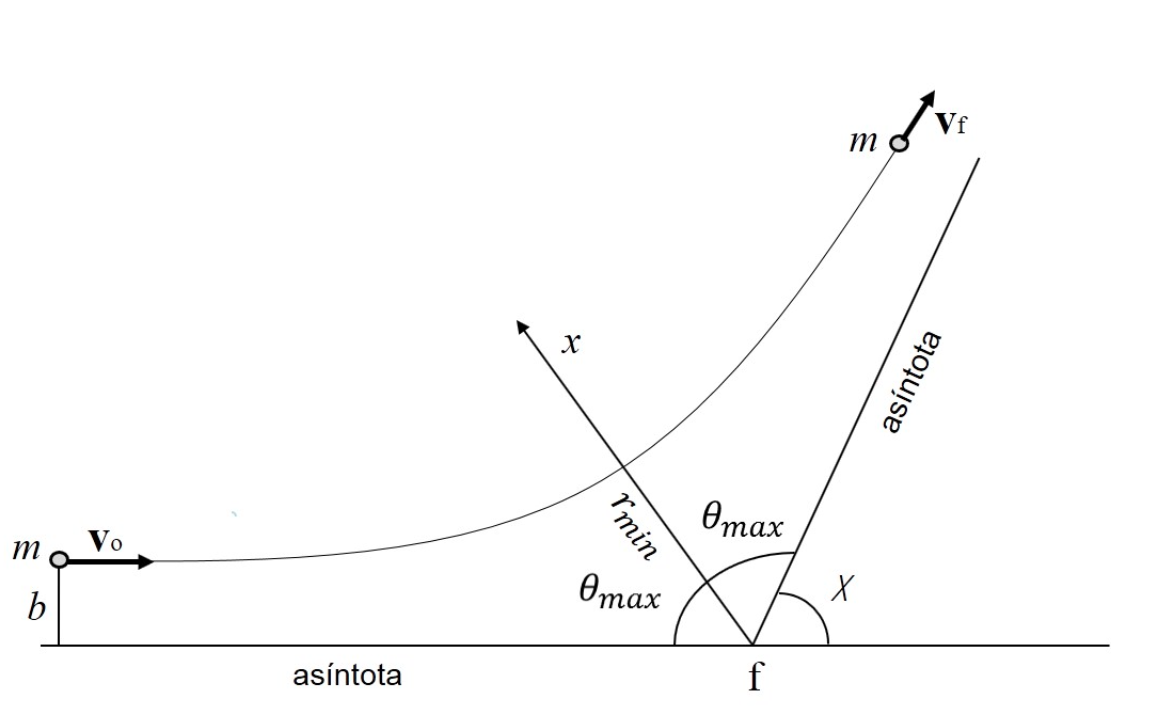
\includegraphics[width=1.8in]{Figuras/Dispersion.png}
   	\end{figure}
	
